\documentclass[11pt]{article}
\usepackage[margin=2.4cm]{geometry}
\usepackage[T1]{fontenc}
\usepackage[utf8]{inputenc}
\usepackage{charter}
\usepackage{microtype}
\usepackage{graphicx}
\usepackage{booktabs}
\usepackage{xcolor}
\usepackage{hyperref}
\usepackage{caption}
\hypersetup{colorlinks=true, linkcolor=black, citecolor=black, urlcolor=blue!50!black}
\captionsetup{font=small, labelfont=bf}
\setlength{\parskip}{0.35em}

\title{Epistemic Bridges\\[0.3em]\large How much of the space of human connections do language models reach?}
\author{Sofia Gallego\\ CosmoVentures, Paris}
\date{AI $\times$ Epistemics Research Sprint, Apart Research, November 2026}

\begin{document}
\maketitle

\begin{abstract}
Give a room of monkeys typewriters and infinite time, and one day they will type Shakespeare, together with a mountain of noise. Creativity lives somewhere between that noise and the cliché: a connection that surprises and still makes sense. This work asks where language models sit between those two ends, compared with people.

To find out, Bridges, a short game, asks people to link two simple ideas, like a bee and a mirror, or salt and a clock, in any way they like. 21 players wrote 109 bridges. The same pairs then went to 13 open language models released between 2019 and 2025, with no persona, with reasoning personas, with creative personas and at different temperatures, for 27{,}720 AI bridges in total.

With both sides in hand, the human answers draw a map of where people go, and each model is placed on it with two numbers, with no AI judging anything: how many of its answers land on the map, and how much of the map it reaches.

Seen this way, another group of players reaches about two thirds of the map and stays on it about as often, and no model gets close to both. The oldest models reach most of the map, mostly by noise. Chat training then closes it: the same 7B model reaches 54\% of the human map before chat training and 8\% after, and the newest model tested, Qwen3 8B, reaches 2\%. From there, personas for reasoning change little, while creative personas taken from how people connect ideas (an ordinary life, a memory, a playful mood) open the map again, about as far as more randomness does, and much further on the newest model. What remains out of reach for every model are personal memories, small everyday scenes and play with words.
\end{abstract}

\section{Introduction}

People are good at connecting distant ideas, and much of brainstorming and discovery happens in those connections. More and more of that thinking now passes through AI tools, which learn from what is already written. If those tools pull everyone toward the same connections, the space of ideas a group can reach becomes smaller. Studies on writing and ideas already point that way: help from AI can improve each person's ideas and still make a group's ideas more alike \cite{doshi2024,anderson2024}.

That worry is the starting point for a larger project: tools that keep the space open, such as a map of ideas that leaves room for contrast and shows how ideas relate (\href{https://mapideas.org}{mapideas.org}). Before building such tools, though, the space itself needs to be visible. So the sprint asks one precise question:

\begin{quote}
\emph{Do the connections language models make between two ideas cover less ground than the ones people make? And how does that change with the age of the model, its size, chat training, personas and temperature?}
\end{quote}

To keep the question clean, the pairs are simple and universal on purpose. Nobody needs to know a topic to play, so the game measures the act of connecting itself, in five languages. Contested ideas, where everyone thinking alike costs more, are the natural next step once the method works.

Answering the question took four pieces, which are also what this work brings:
\begin{itemize}\setlength\itemsep{0.1em}
\item Bridges, an open game that collects free connections between ideas (\href{https://mapideas.org/bridges}{mapideas.org/bridges});
\item a simple way to see how much of the human map a model reaches, with published methods and no AI judge \cite{kynkaanniemi2019};
\item a first look at 13 open models from 2019 to 2025, with reasoning personas, creative personas and a temperature sweep;
\item a description of the human bridges that no model reaches.
\end{itemize}
All code and all AI answers are public at \href{https://github.com/nefinia/epistemic-bridges}{github.com/nefinia/epistemic-bridges}.

\section{Where this comes from}

The game itself is old. In 1879 Lewis Carroll asked readers to turn \textsc{head} into \textsc{tail} one letter at a time. A century later, Koestler described creativity in similar terms, as two unrelated frames of thought meeting \cite{koestler1964}. Psychology turned the idea into tests: the Remote Associates Test asks for the one word that links three distant ones \cite{mednick1962}, and studies of word pairs like ``zebra clam'' looked at how people join two concepts, through a shared property or a relation \cite{wisniewski1997}. Some of these studies also watched people over time. Word association lists go back to 1910, and between 1910 and 1952 people's answers became more alike \cite{jenkins1960}, an early sign that a culture can narrow how people connect. Closer to today, people moving through Wikipedia from one article to another pass through a few central hubs \cite{west2012}, and a daily web game, Linxicon, asks players to link two random words through a chain of single words. Bridges builds on this tradition with an open form, the direction of the arrow kept, and people and AI on the same pairs.

Measuring such connections has its own history. The Divergent Association Task scores how far apart ten words are \cite{olson2021}, and was recently used to compare about 100{,}000 people with language models \cite{bellemare2026}. Ecology offers a way to count diversity as an effective number of different answers \cite{jost2006,friedman2023}. On the AI side, chat training is known to make answers less varied \cite{kirk2024}, and two simple prompts are known to push back: personas of ordinary people \cite{deng2026} and asking a model to think step by step \cite{meincke2024}. This project also grows from earlier work on \emph{false epistemic redundancy}, where AI personas that looked different shared the same blind spots. Here the same question moves from finding answers to connecting ideas.

\section{How it works}

\paragraph{The game.} Everything starts with the players. Two ideas appear, joined by a dashed arrow, and the player writes how to get from one to the other, in any form: a sentence, a chain of words, a memory. Up to three stepping stones can be added. Six core pairs go to everyone, from two concrete things to two abstract ones: bee $\to$ mirror, salt $\to$ clock, river $\to$ secret, spider $\to$ melody, forgetting $\to$ festival, distance $\to$ habit. Each player sees each pair in one direction, and both directions get the same number of players. More pairs are optional, and a ten-word warm-up comes first. An AI bridge can be shown, only if the player asks for it. The game runs in English, French, Spanish, Italian and German, with no account, and stores no name, IP address or location.

\paragraph{The players.} The game was shared during the sprint, and between 25 October and 14 November 2026, 21 players wrote 109 bridges: 87 in English, 20 in Spanish and 2 in French. To compare like with like, the analysis uses the 80 English answers to the core pairs, from 15 players. A typical answer has 9 words and takes about a minute. Most players who answered the optional questions use AI every day and work in engineering; a few work in the arts, health or social sciences, and one never uses AI. One detail of the setting changed along the way: the welcome text went from ``Short or long, any way you like'' to ``Any connection works, short or long'', and 41 answers came after the change.

\paragraph{The models.} The same pairs then went to 13 open models, run on Modal (Table~\ref{tab:models}). Two are base models from before chat training, GPT-2 XL (2019) and GPT-J 6B (2021), which simply continue text. The others are chat models from 2023 to 2025, most of them around 7 billion parameters, plus the Qwen2.5 family from 0.5 to 14 billion and the base Qwen2.5 7B, so that size and chat training can each be seen on their own. Every model got exactly the text the players see.

\paragraph{The conditions.} Each model first answered as it is: each pair, direction and language 10 times, with no persona, at temperature 1.0. Chat models then answered again with the four reasoning personas from false epistemic redundancy, written by Anya Habana: a causal mechanist, an analogical thinker, a teleological analyst and a dialectical thinker. Since those personas were built for investigating, five models also answered with creative conditions, built from the ways players connected ideas:
\begin{itemize}\setlength\itemsep{0.1em}
\item ways of connecting: association, story, memory, senses, wordplay;
\item moods: playful, dreamy, a child's eyes;
\item an ordinary life drawn at random from 30 short sketches, such as ``a 62-year-old fisherwoman in La Serena who mends her own nets'';
\item a small random constraint (``pass through something soft''), and thinking step by step.
\end{itemize}
Finally, to compare personas with plain randomness, two models ran with no persona at temperatures from 0.4 to 2.0. Temperature is how much randomness a model adds when it writes.

\paragraph{The measures.} With all the answers collected, they need to be compared without anyone grading them, and no AI grades any answer here. Each answer is read between its two ideas (``salt \emph{[answer]} a clock''), cut to its first 40 words so long answers gain nothing from length, and placed in a space of meaning by a small embedding model (all-MiniLM-L6-v2), where close answers say similar things.

In that space, the human answers to each pair draw the map: a small circle around each human answer, as wide as the distance to its third closest human neighbour. Every model can then be described with two numbers \cite{kynkaanniemi2019}:
\begin{itemize}\setlength\itemsep{0.1em}
\item \textbf{On the map} (precision): the share of a model's answers that fall inside some human circle, or how close the model stays to what people write;
\item \textbf{Map reached} (recall): the share of human answers that the model also reaches, or how much of the human space it covers.
\end{itemize}
To be fair to the smaller human sample, both are computed with as many model answers as there are human answers for that pair, averaged over 30 random draws, then over the six pairs. Two more numbers complete the picture: how many really different answers a group gives, per answer (the Vendi score \cite{friedman2023}), and how often a group takes the most common human bridge, such as the hourglass for salt and clock or walking for distance and habit. As a check, every result was computed again with two other embedding models and with a shorter 15-word cut.

\section{What came out}

\begin{figure}[t]
\centering
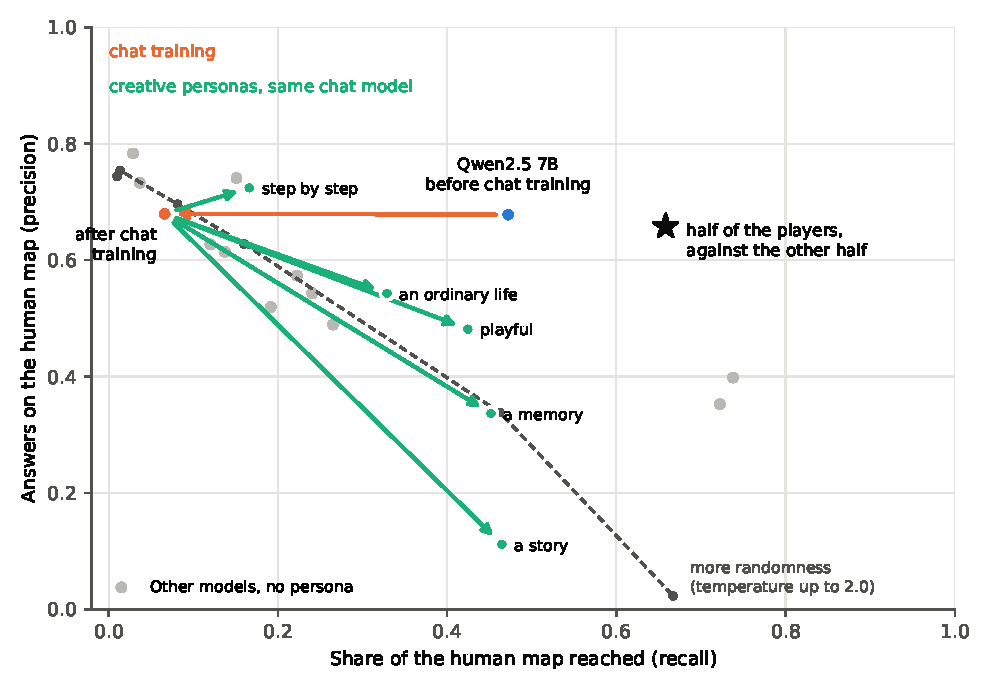
\includegraphics[width=0.86\linewidth]{figs/fig0_money.pdf}
\caption{The whole story on one model. Half of the players draw the map; the star is the other half. Qwen2.5 7B before chat training (blue) reaches far. After chat training (orange) it stays in a small corner. Creative personas on the same chat model (green) open the map again. The dashed line is the same chat model with more and more randomness. Grey dots: the other models with no persona. Here every group is placed against half of the players, so the numbers are a little lower than in Table~\ref{tab:models}.}
\label{fig:money}
\end{figure}

Figure~\ref{fig:money} gathers the whole story on one model. Another group of players reaches about two thirds of the human map and stays on it about as often, and no model comes close to that point. The rest of this section follows the figure step by step, from the oldest models to the creative personas.

\begin{table}[t]
\centering\small
\begin{tabular}{lrrrrrrr}
\toprule
Model & Year & Size (B) & Words & On the map & Map reached & Different & Hub \\
\midrule
People (15 players) & & & 9 & & & 0.27 & 0.33 \\
\midrule
GPT-2 XL (base) & 2019 & 1.5 & 14 & 0.40 & 0.72 & 0.36 & 0.05 \\
GPT-J (base) & 2021 & 6 & 17 & 0.32 & 0.71 & 0.37 & 0.05 \\
Zephyr & 2023 & 7 & 125 & 0.55 & 0.20 & 0.20 & 0.41 \\
Vicuna & 2023 & 7 & 105 & 0.81 & 0.22 & 0.16 & 0.42 \\
Phi-3 mini & 2024 & 3.8 & 142 & 0.53 & 0.28 & 0.21 & 0.48 \\
OLMo 2 & 2024 & 7 & 172 & 0.65 & 0.16 & 0.19 & 0.53 \\
Qwen2.5 & 2024 & 0.5 & 170 & 0.50 & 0.32 & 0.22 & 0.20 \\
Qwen2.5 & 2024 & 1.5 & 169 & 0.60 & 0.30 & 0.20 & 0.36 \\
Qwen2.5 & 2024 & 3 & 172 & 0.60 & 0.17 & 0.19 & 0.39 \\
Qwen2.5 (base) & 2024 & 7 & 34 & 0.68 & 0.54 & 0.23 & 0.23 \\
Qwen2.5 & 2024 & 7 & 172 & 0.69 & 0.08 & 0.16 & 0.48 \\
Qwen2.5 & 2024 & 14 & 174 & 0.74 & 0.03 & 0.16 & 0.47 \\
Qwen3 & 2025 & 8 & 155 & 0.81 & 0.02 & 0.15 & 0.51 \\
\bottomrule
\end{tabular}
\caption{Models with no persona, English, temperature 1.0. Words: typical length of the full answer. On the map: share of answers inside the human space. Map reached: share of the human space the model reaches. Different: really different answers per answer. Hub: share of answers taking the most common human bridge.}
\label{tab:models}
\end{table}

\paragraph{The oldest models reach far by chance. Chat models stay close and small.} The first step is the models with no persona, each shown as one point in Figure~\ref{fig:pr}. GPT-2 and GPT-J reach about 70\% of the human map, yet only a third of their answers land on it: the monkeys at the typewriters. Chat models show the opposite pattern. They land on the map much more often and reach much less of it. Their answers are also more alike than people's (0.15 to 0.22 different answers per answer, against 0.27 for people), and they take the most common bridge more often (41\% to 53\%, against 33\% for people).

\begin{figure}[t]
\centering
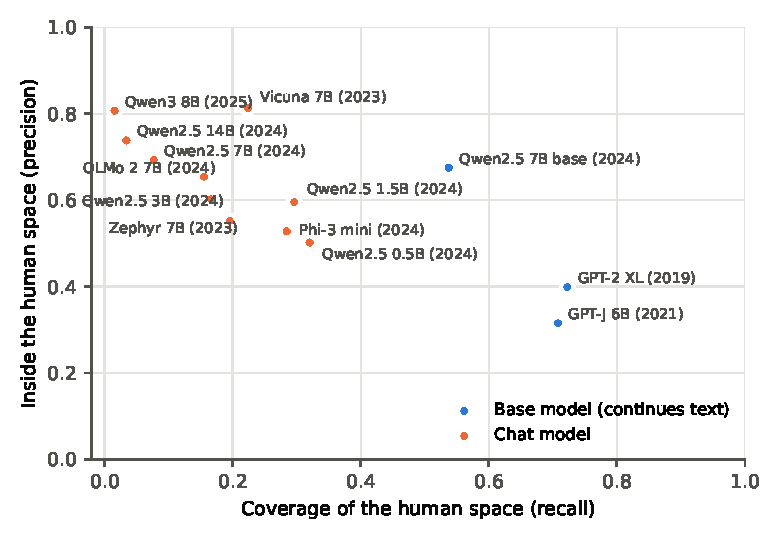
\includegraphics[width=0.72\linewidth]{figs/fig1_precision_recall.pdf}
\caption{Each model with no persona. Across: how much of the human map it reaches. Up: how many of its answers land on the map. Base models in blue, chat models in orange.}
\label{fig:pr}
\end{figure}

\paragraph{Chat training is where the map closes.} Since old base models and new chat models differ in many ways at once, the clearest case keeps everything else the same: Qwen2.5 7B before and after chat training. The share of the map it reaches drops from 54\% to 8\%, while the share of answers on the map stays almost the same (68\% and 69\%). Size adds to the effect. Inside the Qwen2.5 chat family, bigger models reach less, from 32\% at 0.5 billion parameters to 3\% at 14 billion (Figure~\ref{fig:scale}), and the newest model, Qwen3 8B, stays on the map most often of all chat models while reaching the least of it, 2\%. The pattern does not depend on the ruler: with the two other embedding models and the shorter cut, Qwen2.5 14B and Qwen3 8B reach between 0\% and 4\% in every setting, and the 7B base model between 45\% and 69\%.

\begin{figure}[t]
\centering
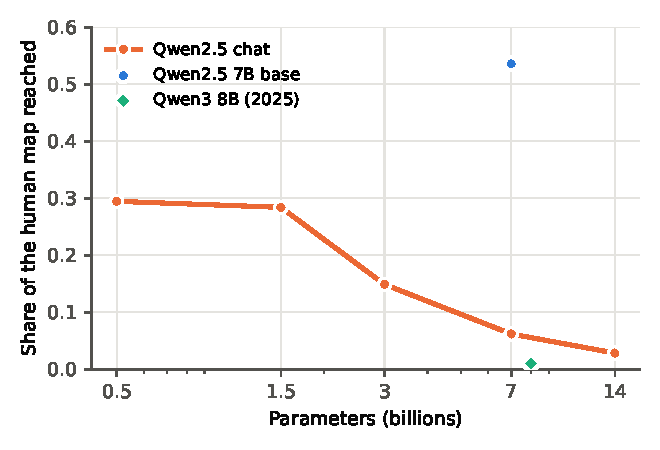
\includegraphics[width=0.55\linewidth]{figs/fig2_scale.pdf}
\caption{Share of the human map reached by the Qwen2.5 chat family at each size, by the same 7B model before chat training, and by the newer Qwen3 8B.}
\label{fig:scale}
\end{figure}

\paragraph{Reasoning personas change little. Creative ones open the map.} If chat training closes the map, the next question is whether a persona can open it again. The four reasoning personas from false epistemic redundancy barely do: they move the share reached by $-3$ to $+2$ points on average (Figure~\ref{fig:conditions}). Every creative condition, in contrast, raises it. The largest gains come from an ordinary life ($+37$ points), a story ($+37$), a memory ($+34$) and a playful mood ($+31$), and on Qwen3 8B the ordinary life takes the share reached from 5\% to 44\%. This opening has a price, since fewer answers land on the map, most of all with \emph{story}, which drops to 10\% on two models. Thinking step by step sits at the careful end: a smaller gain ($+15$ points), with answers still close to people's (57\% to 88\% on the map).

\begin{figure}[t]
\centering
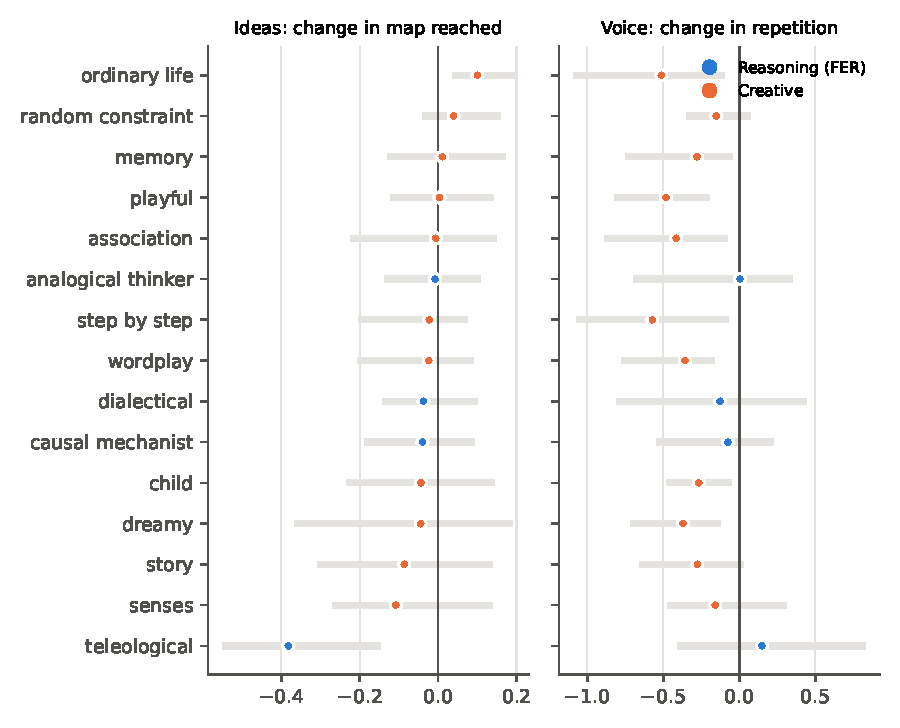
\includegraphics[width=0.62\linewidth]{figs/fig3_conditions.pdf}
\caption{Change in the share of the human map reached, against the same model with no persona. Dot: average. Bar: range across models. Reasoning personas on 10 chat models, creative conditions on 5.}
\label{fig:conditions}
\end{figure}

\paragraph{Personas and randomness open the map about as far.} That price raises a fair doubt: maybe the creative personas only add noise, which plain randomness could do too. Temperature is the monkey dial that tests this. On Qwen2.5 7B, raising it to 1.6 takes the share reached to 45\%, and to 67\% at 2.0, while the share on the map falls to 32\% and then 2\% (dashed line in Figure~\ref{fig:money}). Against that line, an ordinary life and a playful mood sit a little above it, a memory sits on it, and a story falls below it. On Qwen3 8B the difference is larger: temperature hardly moves anything until 2.0 (19\%), while an ordinary life and a memory reach 44\% and 31\%, with at least 44\% of answers on the map. So creative personas are at least as good as randomness at opening the map, and on the newest model much better.

\paragraph{What no model reaches.} Even with every persona and temperature together, some human bridges stay far from all AI answers, and looking at them shows what is missing. The sample is small, so they are described here and never quoted, to keep players from being recognised. The farthest bridges are personal: a wish kept secret, a place from childhood, an object reused in a garden, an afternoon at the sea. After them come an old meaning of a word, and play with the letters or the sound of the words themselves. One more detail matters for measuring: two players, hours apart, found the same rare connection for one pair. A connection can be rare and still shared, and a good measure of diversity should keep it.

\section{What it suggests}

Put together, these steps tell one story. Chat training is the step where the space closes, since base models, old and new, reach much more of the human map than chat models of the same size. Among chat models, the newest and largest are the most reliably sensible and the narrowest, which turns the worry about everyone thinking alike into numbers. Yet the space opens again at little cost, with framings taken from how people really connect ideas: a life, a memory, a story, a mood. The blind spots point the same way, because what the models miss is memory, place and play, the very things the strongest creative conditions bring in.

For tools that help people think, this suggests offering several voices, each drawn from a human way of connecting, and showing how much ground they cover together. A map of ideas is one form such a tool could take.

\section{Limits}

These results come from a first test, and its limits shape how far they go. The human sample is small: 15 players for the English core pairs, mostly engineers who use AI every day, found through AI safety communities. The human map is therefore narrow, and every share reached is relative to it. Players also saw one of two welcome texts. The measures have limits of their own. ``On the map'' measures closeness to what people wrote, which is only a stand-in for making sense, so blind ratings by people, with agreement between raters, are the next check. Model answers are much longer than human ones; every answer was cut to 40 words and read between its two ideas, and a 15-word cut was checked too, but length and style may still play a part, and the embedding models learned from text much like what chat models write. Finally, the choice of models and conditions is narrow. Only open models were tested, mostly one family for size, and one model (Falcon 7B) failed to run. The creative conditions were designed after seeing the first answers, so they borrow the styles, never the texts. Six pairs of simple ideas are a narrow task, and contested ideas are the natural next test.

\appendix
\section{Dual use and ethics}

A way to measure how much of the human map a model reaches could also become a training target, used to make models more varied and inventive, which is a capability. The added risk looks small: every measure here is already published, and the new part is the human baseline. One risk is worth naming: if reaching the map became a target, models could learn to look diverse without being more useful. The measures are offered for watching how models change, and are kept away from training. Players took part anonymously after a consent screen. No name, IP address or location is stored. Page visits are counted only as daily totals per country. Voice answers are transcribed and never stored. Player answers stay out of the public repository, and no answer is quoted in this report, since a small sample makes answers easy to recognise.

\section{What existed before the sprint}

The Bridges game, built before 13 November 2026 (\href{https://github.com/nefinia/themap}{nefinia/themap}), and from false epistemic redundancy the four reasoning personas, the Modal server and the clustering settings. The model runs, the creative conditions, the measures, the analysis and this report were made during the sprint.

\begin{thebibliography}{99}\small
\bibitem{anderson2024} B.~R. Anderson, J.~H. Shah, M.~Kreminski. Homogenization effects of large language models on human creative ideation. \emph{Creativity and Cognition}, 2024.
\bibitem{bellemare2026} A.~Bellemare-Pepin et al. Divergent creativity in humans and large language models. \emph{Scientific Reports}, 2026.
\bibitem{deng2026} Y.~Deng, M.~Brucks, O.~Toubia. Examining and addressing barriers to diversity in LLM-generated ideas. 2026.
\bibitem{doshi2024} A.~R. Doshi, O.~P. Hauser. Generative AI enhances individual creativity but reduces the collective diversity of novel content. \emph{Science Advances} 10(28), 2024.
\bibitem{friedman2023} D.~Friedman, A.~B. Dieng. The Vendi score: a diversity evaluation metric for machine learning. \emph{TMLR}, 2023.
\bibitem{jenkins1960} J.~J. Jenkins, W.~A. Russell. Systematic changes in word association norms: 1910--1952. \emph{Journal of Abnormal and Social Psychology} 60, 1960.
\bibitem{jost2006} L.~Jost. Entropy and diversity. \emph{Oikos} 113(2), 2006.
\bibitem{kirk2024} R.~Kirk et al. Understanding the effects of RLHF on LLM generalisation and diversity. \emph{ICLR}, 2024.
\bibitem{koestler1964} A.~Koestler. \emph{The Act of Creation}. Hutchinson, 1964.
\bibitem{kynkaanniemi2019} T.~Kynkäänniemi, T.~Karras, S.~Laine, J.~Lehtinen, T.~Aila. Improved precision and recall metric for assessing generative models. \emph{NeurIPS}, 2019.
\bibitem{mednick1962} S.~A. Mednick. The associative basis of the creative process. \emph{Psychological Review} 69(3), 1962.
\bibitem{meincke2024} L.~Meincke, E.~Mollick, C.~Terwiesch. Prompting diverse ideas: increasing AI idea variance. 2024.
\bibitem{olson2021} J.~A. Olson, J.~Nahas, D.~Chmoulevitch, S.~J. Cropper, M.~E. Webb. Naming unrelated words predicts creativity. \emph{PNAS} 118(25), 2021.
\bibitem{west2012} R.~West, J.~Leskovec. Human wayfinding in information networks. \emph{WWW}, 2012.
\bibitem{wisniewski1997} E.~J. Wisniewski. When concepts combine. \emph{Psychonomic Bulletin \& Review} 4(2), 1997.
\end{thebibliography}

\end{document}
